\documentclass{standalone}
\usepackage{tikz}
\usepackage{ctex,siunitx}
\setCJKmainfont{Noto Serif CJK SC}
\usepackage{tkz-euclide}
\usepackage{amsmath}
\usetikzlibrary{patterns, calc,3d}
\usetikzlibrary {decorations.pathmorphing,decorations.pathreplacing,decorations.shapes}
\begin{document}
\small
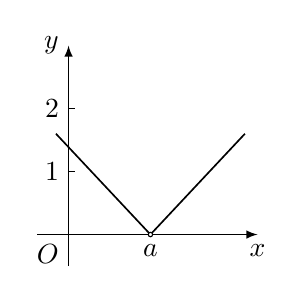
\begin{tikzpicture}[>=latex,scale=0.8]
  \draw[->](-0.5,0)--(3,0)node[below]{$x$};
  \draw[->](0,-0.5)--(0,3)node[left]{$y$};
  \node at (0,0)[below left]{$O$};
  \draw[semithick](-0.2,1.6)--(1.3,0)--(2.8,1.6);
  \foreach \y in {1,2}
  {
    \draw[very thin](0.1,\y)--(0,\y)node[left]{$\y$};
  }
  \draw[fill=white](1.3,0)circle(1.0pt)node[below]{$a$};
\end{tikzpicture}
\end{document}